% Created 2016-08-17 Wed 14:38
\documentclass[tikz]{standalone}

\usepackage[utf8]{inputenc}
\usepackage[T1]{fontenc}
\usepackage{helvet}
\usepackage{../../templates/msc}

\renewcommand{\familydefault}{\sfdefault}

\tikzset{
every picture/.style={
line width=1pt
}}

\usepackage{tikz}
\author{Holger Karl}
\date{\today}
\title{}


\begin{document}
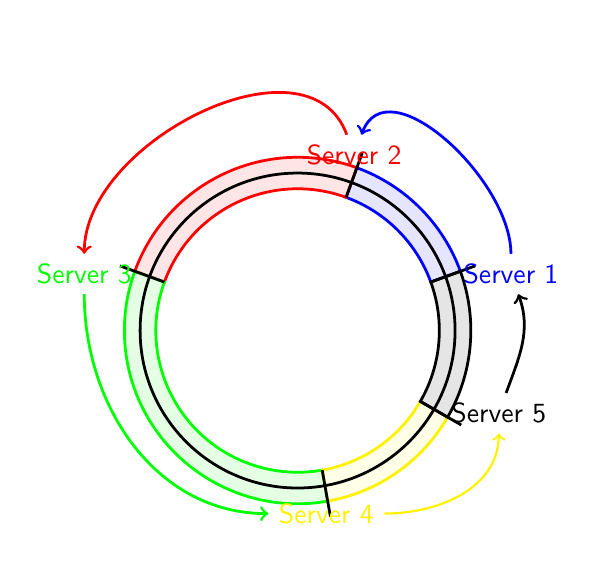
\begin{tikzpicture}[auto, 
block/.style = {rectangle, draw=black, thick, align=left}]

% server: 20, 70, 160, 280, 330 

\draw [blue, fill=blue!10] (20:1.8cm) arc (20:70:1.8cm)
--++ (70:0.4cm)  arc (70:20:2.2cm) -- cycle;

\draw [red, fill=red!10] (70:1.8cm) 
arc (70:160:1.8cm)
--++ (160:0.4cm)  
arc (160:70:2.2cm) -- cycle;

\draw [green, fill=green!10] (160:1.8cm) 
arc (160:280:1.8cm)
--++ (280:0.4cm)  
arc (280:160:2.2cm) -- cycle;

\draw [yellow, fill=yellow!10] (280:1.8cm) 
arc (280:330:1.8cm)
--++ (330:0.4cm)  
arc (330:280:2.2cm) -- cycle;

\draw [black, fill=black!10] (330:1.8cm) 
arc (330:20+360:1.8cm)
--++ (20+360:0.4cm)  
arc (20+360:330:2.2cm) -- cycle;

\draw (0,0) circle (2cm);

\draw (20:1.8cm)  -- node [right, blue] (s1)  {Server 1} (20:2.4cm); 
\draw (70:1.8cm)  -- node [above, red] (s2)  {Server 2} (70:2.4cm); 
\draw (160:1.8cm)  -- node [left, green]  (s3) {Server 3} (160:2.4cm); 
\draw (280:1.8cm)  -- node [below, yellow]  (s4) {Server 4} (280:2.4cm); 
\draw (330:1.8cm)  -- node [right, black]  (s5) {Server 5} (330:2.4cm); 


\draw [blue, ->] (s1) to[out=90, in=70] (s2); 
\draw [red, ->] (s2) to[out=110, in=90] (s3); 
\draw [green, ->] (s3) to[out=270, in=180] (s4); 
\draw [thick,yellow, ->] (s4) to[out=0, in=270] (s5); 
\draw [->] (s5) to[out=70, in=290] (s1);
 
\end{tikzpicture}

%-----------

\begin{tikzpicture}
\foreach \a [count=\ai] in {20, 70, 160, 280, 330}{
  \draw (\a:1.8cm) -- (\a:2.2cm); 
  \node (s\ai) at (\a:2.4cm)  {S \ai};
}

\foreach \a/\b/\ai/\bi in {20/70/1/2, 70/160/2/3, 160/280/3/4, 280/330/4/5, 330/380/5/1}{
  \draw [->,dashed] (s\ai) to[out=\a+20, in=\b-20] (s\bi);
}

\draw (0,0) circle (2cm);
\end{tikzpicture}

%-------------------


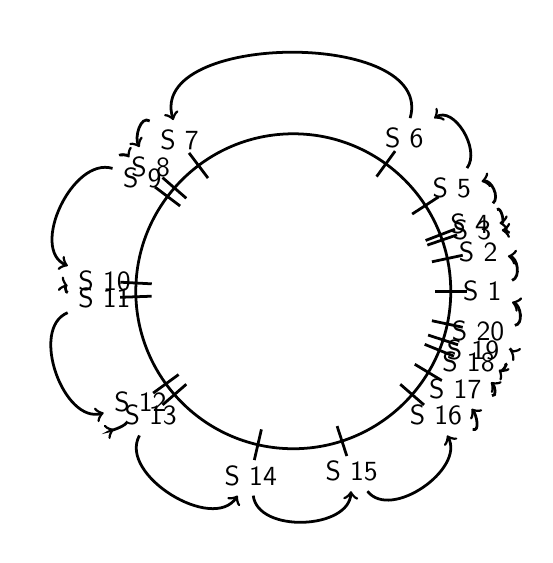
\begin{tikzpicture}
% lilsts: 
% r1 =  [0, 12, 19, 21, 33, 54, 127, 139, 143, 177, 182, 216, 221, 257, 288, 319, 329, 338, 342, 348] 
% r2 = r1[1:] + r1[:1]
% rr = list(zip(r1, r2))
% [ "{}/{}/{}/{}".format(a[0], a[1], i+1, (i+2)%20) for (i, a) in enumerate(rr)]
% ['0/12/1/2', '12/19/2/3', '19/21/3/4', '21/33/4/5', '33/54/5/6', '54/127/6/7', '127/139/7/8', '139/143/8/9', '143/177/9/10', '177/182/10/11', '182/216/11/12', '216/221/12/13', '221/257/13/14', '257/288/14/15', '288/319/15/16', '319/329/16/17', '329/338/17/18', '338/342/18/19', '342/348/19/0', '348/0/20/1']

\foreach \a [count=\ai] in {0, 12, 19, 21, 33, 54, 127, 139, 143, 177, 182, 216, 221, 257, 288, 319, 329, 338, 342, 348}{
  \draw (\a:1.8cm) -- (\a:2.2cm); 
  \node (s\ai) at (\a:2.4cm)  {S \ai};
}

\foreach \a/\b/\ai/\bi in {0/12/1/2, 12/19/2/3, 19/21/3/4, 21/33/4/5, 33/54/5/6, 54/127/6/7, 127/139/7/8, 139/143/8/9, 143/177/9/10, 177/182/10/11, 182/216/11/12, 216/221/12/13, 221/257/13/14, 257/288/14/15, 288/319/15/16, 319/329/16/17, 329/338/17/18, 338/342/18/19, 342/348/19/20, 348/0/20/1}{
  \draw [->] (s\ai) to[out=\a+20, in=\b-20] (s\bi);
}

\draw (0,0) circle (2cm);
\end{tikzpicture}

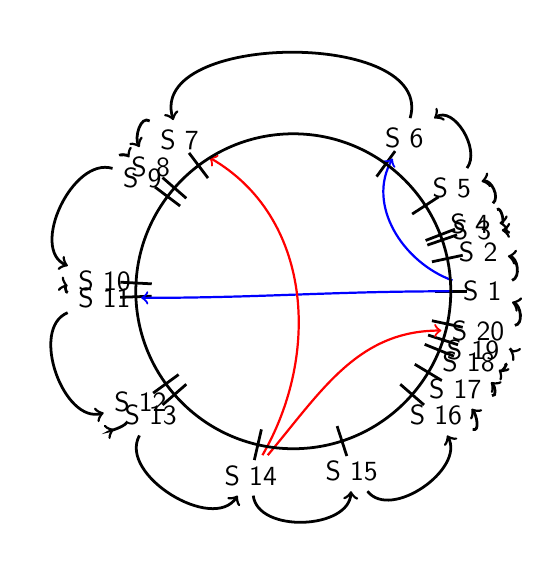
\begin{tikzpicture}
% lilsts: 
% r1 =  [0, 12, 19, 21, 33, 54, 127, 139, 143, 177, 182, 216, 221, 257, 288, 319, 329, 338, 342, 348] 
% r2 = r1[1:] + r1[:1]
% rr = list(zip(r1, r2))
% [ "{}/{}/{}/{}".format(a[0], a[1], i+1, (i+2)%20) for (i, a) in enumerate(rr)]
% ['0/12/1/2', '12/19/2/3', '19/21/3/4', '21/33/4/5', '33/54/5/6', '54/127/6/7', '127/139/7/8', '139/143/8/9', '143/177/9/10', '177/182/10/11', '182/216/11/12', '216/221/12/13', '221/257/13/14', '257/288/14/15', '288/319/15/16', '319/329/16/17', '329/338/17/18', '338/342/18/19', '342/348/19/0', '348/0/20/1']

\foreach \a [count=\ai] in {0, 12, 19, 21, 33, 54, 127, 139, 143, 177, 182, 216, 221, 257, 288, 319, 329, 338, 342, 348}{
  \draw (\a:1.8cm) -- (\a:2.2cm); 
  \node (s\ai) at (\a:2.4cm)  {S \ai};
}

\foreach \a/\b/\ai/\bi in {0/12/1/2, 12/19/2/3, 19/21/3/4, 21/33/4/5, 33/54/5/6, 54/127/6/7, 127/139/7/8, 139/143/8/9, 143/177/9/10, 177/182/10/11, 182/216/11/12, 216/221/12/13, 221/257/13/14, 257/288/14/15, 288/319/15/16, 319/329/16/17, 329/338/17/18, 338/342/18/19, 342/348/19/20, 348/0/20/1}{
  \draw [->] (s\ai) to[out=\a+20, in=\b-20] (s\bi);
}

% and direct links: 
\draw [->, blue, thick] (s1) to[out=180, in=0] (s11); 
\draw [->, blue, thick] (s1) to[out=160, in=240] (s6); 

\draw [->, red, thick] (s14) to[out=60, in=330] (s7); 
\draw [->, red, thick] (s14) to[out=50, in=180] (s20); 


\draw (0,0) circle (2cm);
\end{tikzpicture}


\end{document}